% !TeX program = pdflatex
% !TeX spellcheck = en_US
% !TeX encoding = UTF-8

% update
% v1.13 - 2020-01-15
% - Tanja: change the style.tex: define Black as a color and use it to replace DarkRed (except on the title page)
% - Tanja: change the the titlepage once more 
% - Tanja: change the color code for DarkRed to match the current TU logo sytle
% v1.12 - 2020-01-02
% - Tanja: add new titlepage design and replace all logos with the new one
% v1.11 - 2018-10-15
% - Felix: use Bibtex instead of Biblatex
% v1.10 - 2017-05-30
% - Erik: Refactor the file structure of the front pages
% - Erik: Fix double bibliography entry
% v1.9 - 2017-02-03
% - Dirk: fixed warning: Underfull \hbox (badness 10000) in paragraph main.tex
% - Dirk: fixed warning: "Data encoding is UTF8" -> style.tex 0.1.8
% v1.8 - 2017-02-02
% - Dirk: replaced titlesec package by KOMA-script commands.-> style.tex v0.1.7
% v1.7 - 2014-11-18
% - bib fixes: now using biber instead of bibtex (thanks felix)
% - compile now with pdflatex -> biber -> pdflatex
% v1.6 - 2013-05-13
% - bibliography headers fixed - thanx lorenz lehmann
% - high quality titlepage - thanx thomas graf
% - removed separation of online and offline references -> style 1.4a
% v1.5 - 2013-01-16

\documentclass[twoside,11pt,titlepage,a4paper,english,bibliography=totocnumbered,listof=numbered]{scrbook}
%
% Template Style
% =========================================================================
% = SNET THESIS TEMPLATE STYLE
% =========================================================================

% http://www.snet.tu-berlin.de
% ------------------------
% Adapted version from http://hci.rwth-aachen.de/karrer_thesistemplate (Thorsten Karrer)
% Further adaptions for http://www.elearn.rwth-aachen.de (Sascha Hoellger)
% Further adaptions for SNET @ TU Berlin by Sebastian Göndör (sebastian.goendoer@tu-berlin.de)


% =========================================================================
% = CHANGELOG
% =========================================================================
% [0.1.9]
% - Fixed styling for chapters and toc using Komascript
% - Remove double bibliography TOC entry
%
% [0.1.8]
% - fixed "warning UFT8 is used". biblatex requires ascii encoding; by Dirk
%
% [0.1.7]
% replaced "Titelsec" commands (and whole package) by appropriate KOMA-Script commands; by Dirk
%
% [0.1.6]
% replaced deprecated \rm commands with \rmfamily commands; by Dirk
%
% [0.1.4b]
% backend=biber added in line 139
%
% [0.1.4a]
% title page: image logo sizes and margins adjusted to printable area
% removed separation of online and offline references
%
% [0.1.3]
% wider text body
% added "school" to the titlepage
% paragraph indents
% correctly placed footnote graphics
%
% [0.1.2]
% new titlepage
% some minor fixes
%
% [0.1.1]
% changed titlepage logo
% added listoffigures and listoftables
% excluded abstract from toc
% no (roman) numbering for frontmatter
%
% [0.1]
% adapted version 0.991b from sascha hoellger @ rwth aachen


% =========================================================================
% = MISC
% =========================================================================

\usepackage{a4wide}					%
\usepackage{verbatim}				%
\usepackage[toc,page]{appendix}			%
\usepackage[withpage]{acronym}			%
\usepackage{amsthm}				% Definitions


% =========================================================================
% = COLORS
% =========================================================================

\usepackage{xcolor}					% Colors
\definecolor{LightBlue}{rgb}{0.55,0.55,1}
\definecolor{DarkBlue}{rgb}{0.2,0.2,0.5}
\definecolor{DarkRed}{rgb}{0.7725490196,0.05490196078,0.12549019607} % new TU red
\definecolor{Black}{rgb}{0,0,0}

% =========================================================================
% = PAGE LAYOUT
% =========================================================================

\usepackage{geometry}
\geometry{inner=3cm, outer=2cm, bottom=4cm}

\newcommand{\setwidesite}				% changes the geometry to have less margin
{
	\fancyhfoffset[LE,RO]{0cm}
	\fancyheadoffset[LO,RE]{0cm}
	\fancyfootoffset[RE]{2cm}
	\newgeometry{inner=2cm, outer=2cm, bottom=4cm}
}

\usepackage{style/noindent}				%do not indent at new paragraphs but add a vertical offset

\setlength{\parindent}{4mm}
\setlength{\parskip}{1.5mm }


% =========================================================================
% = TYPESETTING
% =========================================================================

\usepackage[hyphens]{url}				% url
\usepackage{hyphenat}				% hyphenation. use \hyphenation{}

\righthyphenmin=5
\lefthyphenmin=5


% =========================================================================
% = TABLE OF CONTENTS
% =========================================================================

\setcounter{secnumdepth}{4}
\setcounter{tocdepth}{3}

\addtokomafont{disposition}{\rmfamily}


% =========================================================================
% = FONTS
% =========================================================================

\usepackage{mathpazo}
\usepackage[scaled=.95]{helvet}
\usepackage{courier}


% =========================================================================
% = SYMBOLS
% =========================================================================

%\usepackage{gensymb}
\usepackage{textcomp} 				% for \textmu (non-italic $\mu$)
\makeatletter						% this makes "@" a regular letter


% =========================================================================
% = TABLES
% =========================================================================

\usepackage{tabularx}
\usepackage{booktabs}
\usepackage{multirow}
\usepackage{longtable}				% tables spanning over more than one page

%%\setlength{\fboxsep}{0mm}			% spacing between \fbox border and content

\usepackage{amsmath}				% math fonts
\usepackage{amssymb}				% math symbols
\usepackage{setspace}				% line spacing


% =========================================================================
% = BIBILOGRAPHY
% =========================================================================

% 2018-10-16 - changed to use Bibtex instead

%\usepackage[style=numeric,natbib=true,backend=biber]{biblatex}

% apparently no effect?
%\renewcommand{\bibsetup}{
%	\markboth{
%		\MakeUppercase{Bibliography}
%	}{}
%}

%\ifdefined\bibheadingonline
%  \defbibheading{online}{\section*{\bibheadingonline}}
%\else
%  \defbibheading{online}{\section*{Online References}}
%\fi
%\ifdefined\bibheadingoffline
%  \defbibheading{offline}{\section*{\bibheadingoffline}}
%\else
%  \defbibheading{offline}{\section*{Printed References}}
%\fi
%
%\defbibfilter{online}{%
%  \( \type{online} \)}
%
%\defbibfilter{offline}{%
%  \( \not \type{online} \)}
%
%\bibliography{Bibliography}


% =========================================================================
% = LANGUAGE & ENCODING
% =========================================================================

\usepackage[english]{babel}				% \usepackage[ngerman]{babel}

\selectlanguage{english}				% \selectlanguage{ngerman}

\usepackage[T1]{fontenc}
\usepackage[utf8]{inputenc}				% can use native umlauts

% \usepackage[babel,german=quotes]{csquotes}	% provides \enquote{Blupp} => "`Blupp"'
\usepackage[babel,english=american]{csquotes}	% provides \enquote{Blupp} => "`Blupp"'

%\SetCiteCommand{\parencite}			% Changed for biblatex

\usepackage{units}					% unified way of setting values with units

\usepackage{appendix}


% =========================================================================
% = CODE LISTINGS
% =========================================================================

\usepackage{listings}

% Listings Styles from Max

\definecolor{violet}{cmyk}{0.45,0.97,0.27,0.21}
\definecolor{lstblue}{cmyk}{1,0.80,0,0}
\definecolor{lstgreen}{cmyk}{0.71,0.21,0.65,0.22}
\definecolor{bluegrey}{cmyk}{0.56,0.24,0.11,0.05}
\definecolor{javadoc}{cmyk}{0.88,0.59,0,0}
\definecolor{lstgrey}{cmyk}{0.55,0.44,0.42,0.32}

\lstdefinelanguage{SQL}{
     keywords={},
     keywordstyle=\color{bluegrey}\bfseries,
     morekeywords=[2]{CREATE,TABLE,IF,NOT,EXISTS,NULL,SET,DEFAULT,PRIMARY,KEY,COLLATE,CHARACTER,AUTO_INCREMENT,ENGINE,CHARSET},
     keywordstyle={[2]\color{violet}\bfseries},
     otherkeywords={int,varchar,double,text,tinyint},
     sensitive=false,
     morecomment=[l][\color{lstgreen}]{//},
     morecomment=[s][\color{lstgreen}]{/*}{*/},
     morecomment=[s][\color{javadoc}]{/**}{*/},
     morestring=[b]',
     morestring=[b]"
  }
\lstdefinelanguage{PHP}{
     keywords={},
     keywordstyle=\color{bluegrey}\bfseries,
     morekeywords=[2]{static,function,if,return,pow,sin,cos,asin,min,sqrt,int},
     keywordstyle={[2]\color{violet}\bfseries},
     otherkeywords={@param, @returns, @author, @type, @link, @see},
     sensitive=false,
     morecomment=[l][\color{lstgreen}]{//},
     morecomment=[s][\color{lstgreen}]{/*}{*/},
     morecomment=[s][\color{javadoc}]{/**}{*/},
     morestring=[b]',
     morestring=[b]"
  }
\lstdefinelanguage{JavaScript}{
     keywords={},
     keywordstyle=\color{bluegrey}\bfseries,
     morekeywords=[2]{attributes, class, classend, do, empty, endif, endwhile, fail, function, functionend, if, implements, in, inherit, inout, not, of, operations, out, return, set, then, types, while, use},
     keywordstyle={[2]\color{violet}\bfseries},
     otherkeywords={@param, @returns, @author, @type, @link, @see},
     sensitive=false,
     morecomment=[l][\color{lstgreen}]{//},
     morecomment=[s][\color{lstgreen}]{/*}{*/},
     morecomment=[s][\color{javadoc}]{/**}{*/},
     morestring=[b]',
     morestring=[b]"
  }
\lstdefinelanguage{Java}{
     keywords={},
     keywordstyle=\color{bluegrey}\bfseries,
     morekeywords=[2]{abstract,boolean,break,byte,case,catch,char,class,
      const,continue,default,do,double,else,extends,false,final,
      finally,float,for,goto,if,implements,import,instanceof,int,
      interface,label,long,native,new,null,package,private,protected,
      public,return,short,static,super,switch,synchronized,this,throw,
      throws,transient,true,try,void,volatile,while},
     keywordstyle={[2]\color{violet}\bfseries},
     morekeywords=[3]{@SuppressWarnings, @Capability, @Override},
     keywordstyle={[3]\color{lstgrey}},
     otherkeywords={@param, @return, @returns, @author, @link, @see},
     sensitive,
     morecomment=[l]//,
     morecomment=[s]{/*}{*/},
     morecomment=[s][\color{javadoc}]{/**}{*/},
     morestring=[b]",
     morestring=[b]',
  }[keywords,comments,strings]

% some listings styles from Gregor Aisch
% http://vis4.net/blog/2009/09/noch-mehr-sprach-definitionen-fuer-latex-listings/

\lstdefinelanguage{HTML5} {morekeywords={a, abbr, address, area, article, aside, audio, b, base, bb, bdo, blockquote,  body, br, button, canvas, caption, cite, code, col, colgroup, command, datagrid, datalist, dd, del, details, dialog, dfn, div, dl, dt, em, embed, eventsource, fieldset, figure, footer,  form,  h1, h2,  h3,  h4, h5,  h6,  head,  header,  hr, html,  i, iframe,  img,  input,  ins, kbd,  label,  legend,  li,  link,  mark,  map,  menu,  meta,  meter,  nav,  noscript,  object,  ol,  optgroup,  option,  output,  p,  param,  pre,  progress,  q,  ruby,  rp,  rt,  samp,  script,  section,  select,  small,  source,  span,  strong,  style,  sub,  sup,  table,  tbody,  td,  textarea,  tfoot,  th,  thead,  time,  title,  tr,  ul,  var,  video},
sensitive=false, morecomment=[s]{<!--}{-->}, morestring=[b]", morestring=[d]'}

\lstdefinelanguage{CSS} {morekeywords={azimuth,  background-attachment,  background-color,  background-image,  background-position,  background-repeat,  background,  border-collapse,  border-color,  border-spacing,  border-style,  border-top, border-right, border-bottom, border-left,  border-top-color, border-right-color, border-bottom-color, border-left-color,  border-top-style, border-right-style, border-bottom-style, border-left-style,  border-top-width, border-right-width, border-bottom-width, border-left-width,  border-width,  border,  bottom,  caption-side,  clear,  clip,  color,  content,  counter-increment,  counter-reset,  cue-after,  cue-before,  cue,  cursor,  direction,  display,  elevation,  empty-cells,  float,  font-family,  font-size,  font-style,  font-variant,  font-weight,  font,  height,  left,  letter-spacing,  line-height,  list-style-image,  list-style-position,  list-style-type,  list-style,  margin-right, margin-left,  margin-top, margin-bottom,  margin,  max-height,  max-width,  min-height,  min-width,  orphans,  outline-color,  outline-style,  outline-width,  outline,  overflow,  padding-top, padding-right, padding-bottom, padding-left,  padding,  page-break-after,  page-break-before,  page-break-inside,  pause-after,  pause-before,  pause,  pitch-range,  pitch,  play-during,  position,  quotes,  richness,  right,  speak-header,  speak-numeral,  speak-punctuation,  speak,  speech-rate,  stress,  table-layout,  text-align,  text-decoration,  text-indent,  text-transform,  top,  unicode-bidi,  vertical-align,  visibility,  voice-family,  volume,  white-space,  widows,  width,  word-spacing,  z-index},
sensitive=false, morecomment=[s]{/*}{*/}, morestring=[b]", morestring=[d]'}

\lstdefinelanguage{JavaFX} {morekeywords={abstract, after, and, as, assert, at, attribute, before, bind, bound, break, catch, class, continue, def, delete, else, exclusive, extends, false, finally, first, for, from, function, if, import, indexof, in, init, insert, instanceof, into, inverse, last, lazy, mixin, mod, new, not, null, on, or, override, package, postinit, private, protected, public-init, public, public-read, replace, return, reverse, sizeof, static, step, super, then, this, throw, trigger, true, try, tween, typeof, var, where, while, with },
sensitive=false, morecomment=[l]{//}, morecomment=[s]{/*}{*/}, morestring=[b]", morestring=[d]'}

\lstdefinelanguage{MXML} {morekeywords={mx:Accordion, mx:Box, mx:Canvas, mx:ControlBar, mx:DividedBox, mx:Form, mx:FormHeading, mx:FormItem, mx:Grid, mx:GridItem, mx:GridRow, mx:HBox, mx:HDividedBox, mx:LinkBar, mx:Panel, mx:TabBar, mx:TabNavigator, mx:Tile, mx:TitleWindow, mx:VBox, mx:VDividedBox, mx:ViewStack, mx:Button, mx:CheckBox, mx:ComboBase, mx:ComboBox, mx:DataGrid, mx:DateChooser, mx:DateField, mx:HRule, mx:Image, mx:Label, mx:Link, mx:List, mx:Loader, mx:MediaController, mx:MediaDisplay, mx:MediaPlayback, mx:MenuBar, mx:NumericStepper, mx:ProgressBar, mx:RadioButton, mx:RadioButtonGroup, mx:Spacer, mx:Text, mx:TextArea, mx:TextInput, mx:Tree, mx:VRule, mx:VScrollBar, mx:Application, mx:Repeater, mx:UIComponent, mx:UIObject, mx:View, mx:FlexExtension, mx:UIComponentExtension, mx:UIObjectExtension, mx:Fade, mx:Move, mx:Parallel, mx:Pause, mx:Resize, mx:Sequence, mx:WipeDown, mx:WipeLeft, mx:WipeRight, mx:WipeUp, mx:Zoom, mx:EventDispatcher, mx:LowLevelEvents, mx:UIEventDispatcher, mx:CurrencyFormatter, mx:DateFormatter, mx:NumberFormatter, mx:PhoneFormatter, mx:ZipCodeFormatter, mx:CursorManager, mx:DepthManager, mx:DragManager, mx:FocusManager, mx:HistoryManager, mx:LayoutManager, mx:OverlappedWindows, mx:PopUpManager, mx:SystemManager, mx:TooltipManager, mx:CreditCardValidator, mx:DateValidator, mx:EmailValidator, mx:NumberValidator, mx:PhoneNumberValidator, mx:SocialSecurityValidator, mx:StringValidator, mx:ZipCodeValidator, mx:DownloadProgressBar, mx:ArrayUtil, mx:ClassUtil, mx:Delegate, mx:ObjectCopy, mx:URLUtil, mx:XMLUtil, mx:CSSSetStyle, mx:CSSStyleDeclaration, mx:CSSTextStyles, mx:StyleManager, mx:HTTPService, mx:RemoteObject, mx:Service},
sensitive=false, morecomment=[s]{<!--}{-->}, morestring=[b]", morestring=[d]'}

\lstdefinelanguage{LZX} {morekeywords={a, alert, animator, animatorgroup , attribute, audio , axis, axisstyle , b, barchart, basebutton , basebuttonrepeater , basecombobox , basecomponent , basedatacombobox , basedatepicker , basedatepickerday , basedatepickerweek , basefloatinglist , basefocusview , baseform , baseformitem , basegrid , basegridcolumn , baselist , baselistitem , basescrollarrow , basescrollbar , basescrollthumb , basescrolltrack , baseslider , basestyle , basetab , basetabelement , basetabpane , basetabs , basetabsbar , basetabscontent , basetabslider , basetrackgroup , basetree , basevaluecomponent , basewindow , br , button , canvas , chart , chartbgstyle , chartstyle , checkbox , class , columnchart , combobox , command , connection , connectiondatasource , constantboundslayout , constantlayout , datacolumn , datacombobox , datalabel , datamarker , datapath , datapointer , dataselectionmanager , dataseries , dataset , datasource , datastyle , datastylelist , datatip , datepicker , debug , dragstate , drawview , edittext , event , face , floatinglist , font , font , form , frame , grid , gridcolumn , gridtext , handler , hbox , horizontalaxis , hscrollbar , i , image , img , import , include , inputtext , javarpc , label , labelstyle , layout , legend , library , linechart , linestyle , list , listitem , LzTextFormat , menu , menubar , menuitem , menuseparator , method , modaldialog , multistatebutton , node , p , param , piechart , piechartplotarea , plainfloatinglist , plotstyle , pointstyle , pre , radiobutton , radiogroup , rectangularchart , regionstyle , remotecall , resizelayout , resizestate , resource , reverselayout , richinputtext , rpc , script , scrollbar , security , selectionmanager , sessionrpc , simpleboundslayout , simpleinputtext , simplelayout , slider , soap , splash , stableborderlayout , state , statictext , style , submit , swatchview , SyncTester , tab , tabelement , tabpane , tabs , tabsbar , tabscontent , tabslider , Test , TestCase , TestResult , TestSuite , text , textlistitem , tickstyle , tree , u , valueline , valuelinestyle , valuepoints , valuepointstyle , valueregion , valueregionstyle , vbox , verticalaxis , view , view , vscrollbar , webapprpc , window , windowpanel , wrappinglayout , XMLHttpRequest , xmlrpc , zoomarea},
sensitive=false, morecomment=[s]{<!--}{-->}, morestring=[b]", morestring=[d]'}

\lstset{
  numbers=left,
  numberstyle=\tiny,
  numbersep=5pt,
  breaklines=true,
  stepnumber=1,
  tabsize=2,
  basicstyle=\ttfamily\small,
  frame=none,
  numberfirstline=true,
  firstnumber=1,
  keywordstyle=\color{violet}\bfseries,
  ndkeywordstyle=\color{bluegrey}\bfseries,
  identifierstyle=\color{black},
  commentstyle=\color{lstgreen}\ttfamily,
  stringstyle=\color{lstblue}\ttfamily,
  showstringspaces=false
}


% ========================================================================
% = CHANGE LIST DEFINITIONS
% ========================================================================

% change color of item list
\renewcommand{\labelitemi}{\color{Black}$\bullet$}
\renewcommand{\labelitemii}{\color{Black}$\circ$}
\renewcommand{\labelitemiii}{\color{Black}$\ast$}
\renewcommand{\labelitemiv}{\color{Black}$\diamond$}

% change color of enum list
\renewcommand{\labelenumi}{\color{Black}\arabic{enumi}.}
\renewcommand{\labelenumii}{\color{Black}\alph{enumii})}
\renewcommand{\labelenumiii}{\color{Black}\roman{enumiii}.}
\renewcommand{\labelenumiv}{\color{Black}\Alph{enumiv}.}

% change color of description list
\usepackage{enumitem}
\setdescription{font=\color{Black}\rmfamily\itshape}
%\renewenvironment{description}{\list{font=\color{Black}\itshape}}{\endlist}


% ========================================================================
% = FOOTNOTES
% ========================================================================

% change color of footnotes
\renewcommand{\thefootnote}{\color{Black}\arabic{footnote}}

% use nice footnote indentation
\deffootnote[1em]{1em}{1em}{\textsuperscript{\thefootnotemark}\,}


% =========================================================================
% = GRAPHICS AND IMAGES
% =========================================================================

\usepackage{graphicx}
\graphicspath{{images/}}				% path to your image folder

\usepackage{eso-pic}					% needed for the full-face titlepage
\usepackage{chngpage}				% we need this to determine if a figure is on an odd or even page
\usepackage{tikz}					% tikz pictures

% captions of tables and images
\usepackage[hang,small,sf]{caption}
\renewcommand{\captionfont}{\sffamily\small}
\renewcommand{\captionlabelfont}{\bfseries}

\usepackage{float}
\usepackage{placeins}
% \floatstyle{ruled}
%\floatplacement

\renewcommand{\floatpagefraction}{0.85}		% if a figure takes more than 85% of a page it will be typeset on a separate page
\usepackage[it,bf,tight,hang,raggedright]{subfigure}

%\numberwithin{figure}{section}
%\numberwithin{table}{section}


% =========================================================================
% = HEADER
% =========================================================================

\newcommand{\STYLEfootnotetext}
{
  \begin{minipage}
  {.2\textwidth}
    
\includegraphics[width=0.6\textwidth]{images/snet/snet_footer.png}
  \end{minipage}
}

% Change page headers and footers:
\usepackage{calc}
\usepackage{fancyhdr}
\pagestyle{fancy}
\fancyhfoffset[RO,LE]{0.1cm} %{\marginparsep+\marginparwidth}
\fancyhfoffset[RE,LO]{0.1cm}
%\fancyheadoffset[RE,LO]{\hoffset + \oddsidemargin}
\renewcommand{\headrule}{{\color{Black}%
  \hrule width\headwidth height\headrulewidth \vskip-\headrulewidth}}
\fancyhf{}
\fancyhead[RE]{\slshape \nouppercase{\leftmark}}    % Even page header: "page   chapter"
\fancyhead[LO]{\slshape \nouppercase{\rightmark}}   % Odd  page header: "section   page"
\fancyhead[RO,LE]{\bfseries \thepage}

%- \fancyfoot[LE]{\STYLEleftpicture}
%- \fancyfoot[RO]{\STYLErightpicture}
\fancyfoot[LE]{\STYLEfootnotetext}

\renewcommand{\headrulewidth}{1pt}    % Underline headers
\renewcommand{\footrulewidth}{0pt}

% =========================================================================
% = SECTIONS THEMING
% =========================================================================

\newcommand{\allsectionformat}{\color{Black}\rmfamily\normalfont}

% Font style and colors
\addtokomafont{part}{\Huge\allsectionformat}
\addtokomafont{chapter}{\Huge\allsectionformat}
\addtokomafont{section}{\allsectionformat}
\addtokomafont{subsection}{\allsectionformat}
\addtokomafont{subsubsection}{\allsectionformat}
\addtokomafont{paragraph}{\allsectionformat}
\addtokomafont{subparagraph}{\allsectionformat}

% Spacing before and after the section titles
\RedeclareSectionCommand[
  beforeskip=-.75\baselineskip,
  afterskip=.5\baselineskip]{section}

\RedeclareSectionCommand[
  beforeskip=-5\baselineskip,
  afterskip=.5\baselineskip]{chapter}


% =========================================================================
% = TYPESETTING - TWEAKES
% =========================================================================

\addtokomafont{section}{\LARGE}
\addtokomafont{subsection}{\large}

% instead of sloppy
%\tolerance 1414
%\hbadness 1414
%- \tolerance 2414
%- \hbadness 2414
%- \emergencystretch 1.5em
%- \hfuzz 0.3pt
%- \widowpenalty=10000
%- \clubpenalty=10000
%- \brokenpenalty=10000
%- \interlinepenalty=9000 % seitenumbruch im absatz
%- \vfuzz \hfuzz
%- \raggedbottom


% =========================================================================
% =  USER DEFINED COMMANDS
% =========================================================================

\newcommand{\chapterquote}[2]{
    \begin{quotation}
    \begin{flushright}
    \noindent\emph{``{#1}''\\[1.5ex]---{#2}}
    \end{flushright}
    \end{quotation}
}


% custom hyphenation					% add words to this list to prevent hyphenation
\hyphenation{
ASCII
TCP
}

%make readable references
\usepackage[pdftex,pdfpagelabels=true]{hyperref}
\hypersetup{%
	pdftitle={Thesis Title},
	pdfauthor={Thesis Author},
	pdfkeywords={key1, key2, key3},
	pdfsubject={Thesis Subject}
}

% Adding a finite stretch on the page suppresses "Underfull \vbox (badness 10000)" warnings.
\makeatletter
\def\@textbottom{\vskip \z@ \@plus 1pt}
\let\@texttop\relax
\makeatother

\begin{document}

%--------------------------------------------------------------
% FRONT PAGE AND DOCUMENT METADATA
%--------------------------------------------------------------
\frontmatter

\begin{titlepage}
	\AddToShipoutPicture*{
		\put(0,0){
			
\includegraphics[width=\paperwidth,height=\paperheight,keepaspectratio=false]{images/snet/titlepage.pdf}
		}
	}
	\strut
	\hfill
	\begin{center}
	\vspace{1cm}
		\Huge
		\begin{spacing}{.9}
			\textcolor{DarkRed}{\textbf{A middleware for inter-vendor mobile robot communication}}\\
		\end{spacing}
		\vspace{0.8cm}
		\large
		by\\
		\vspace{0.8cm}
		\textbf{Mai Khanh Isabelle Wilhelm}\\
		\vspace{0.8cm}
		\textbf{Matriculation Number 406187}\\
		\vspace{2cm}
	 	A thesis submitted to\\
	 	\vspace{0.5cm}
		Technische Universität Berlin\\
		School IV - Electrical Engineering and Computer Science\\
		Department of Telecommunication Systems\\
		Service-centric Networking\\
		\vspace{0.5cm}
		Master's Thesis\\
		\vspace{2.2cm}
		\today\\
		\vspace{2.0cm}
		\large
		Supervised by:\\
		Prof. Dr. Axel Küpper\\
		\vspace{1cm}
		Assistant supervisor:\\
		M. Sc. Kai Gruntert
		\end{center}
         		%\includegraphics[scale=1.0]{images/watermark.png}
\end{titlepage}

% Clear two pages after the title
\shipout\null
\shipout\null

\chapter*{\LARGE Eidestattliche Erklärung / Statutory Declaration}
Hiermit erkläre ich, dass ich die vorliegende Arbeit selbstständig und eigenhändig sowie ohne unerlaubte fremde Hilfe und ausschließlich unter Verwendung der aufgeführten Quellen und Hilfsmittel angefertigt habe.
\vspace{2em}

\noindent I hereby declare that I have created this work completely on my own and used no other sources or tools than the ones listed.

\vspace{30 mm}
\begin{flushright}

\rule{90mm}{1pt}

Darmstadt, \today \hspace{15 mm} Mai Khanh Isabelle Wilhelm
\end{flushright}

%\chapter*{Acknowledgments}
\label{cha:acknowledgments}

I would like to thank my teddybear...

\chapter*{Abstract}
\label{cha:abstract}

In this thesis, we show that lorem ipsum dolor sit amet.					% EN Abstract
\chapter*{Zusammenfassung}
\label{cha:zusammenfassung}

Hier kommt das deutsche Abstract hin. Wie das geht, kann man wie immer auf Wikipedia nachlesen \url{http://de.wikipedia.org/wiki/Abstract}...	% DE Abstract

\tableofcontents{}

%--------------------------------------------------------------
% MAIN CONTENT
%--------------------------------------------------------------
\mainmatter

%\part{}						% optional: use parts to structure your thesis
\chapter{Introduction}
\label{cha:introduction}


\chapterquote{Technologies that are emerging today will soon be shaping the world tomorrow and well into the future – with impacts to economies and to society at large. Now that we are well into the Fourth Industrial Revolution, it’s critical that we discuss and ensure that humanity is served by these new innovations so that we can continue to prosper.}{Marinette DiChristina, Summer Davos Forum 2019, 01.-03.07.2019}

The idea of Industry 4.0 was first brought to public attention in 2011 as a project to digitize the industry. Cyber-Physical Systems, the Internet of Things, and the Internet of Services are key technologies of Industry 4.0 and enhance the manufacturing process of companies \cite{quadrini_open_2020}. To stay competitive, manufacturing processes have to fulfill requirements such as consistency, cost-effectiveness, flexibility, efficiency, and quality. Those challenges are met by automating the process of manufacturing products \cite{sharma_management_2017, krzhizhanovskaya_autonomous_2020, andreasson_autonomous_2015}. Industry 4.0 aims to increase operational effectiveness and efficiency by automating processes, enabling flexible adjustments during production, as well as lowering material and human resources. Connecting devices and exchanging information between them increases the productivity of a facility.

Mobile robots are machines that use sensors and software to move in their surroundings. They are often used to transport materials or products. Thanks to their flexible and mobile movement, mobile robots can more easily react to changes than traditional industrial robots \cite{krzhizhanovskaya_autonomous_2020, gunthner_internet_2010}. 

Different vendors build mobile robots with different functionalities. Thanks to those, they can be more flexibly used in a production line and complete tasks that single-vendor strategies cannot complete. In addition to increased flexibility, it is of high interest for industries to be vendor-independent to decrease repair and maintenance costs. However, vendors provide their own and proprietary applications and interfaces for mobile robots \cite{sanneman_state_2020}. Hence, using mobile robots from different vendors to profit from their different strengths and functionalities increases the programming costs \cite{lambrecht_control_2011}. Further challenges are missing external interfaces for communication and a lack of documentation. While some vendors of mobile robots provide detailed documentation of the mobile robot’s integration and interfaces, others do not \cite{jepsen_pilot_2020}.

A communication standard for mobile robots is critically important, especially for industries using multi-vendor mobile robots solutions \cite{nayyar_challenges_2020}. It is similar to human language in which every language defines unique terms. Hence, people using the same language understand each other. The task the mobile robot should perform should be understood by the mobile robot and the controlling application. Figure ~\ref{fig:introduction__humanstandard} on page ~\pageref{fig:introduction__humanstandard} represents this human analogy of a communication standard. Whereas the red and the yellow rectangles represent the use of two different languages and therefore the use of a non-compatible interface, the green rectangles represent the use of one language (compatible interface). To use mobile robots from different vendors a standard that guarantees a compatible use of interfaces is needed.

\begin{figure}[!ht]
	\centering
	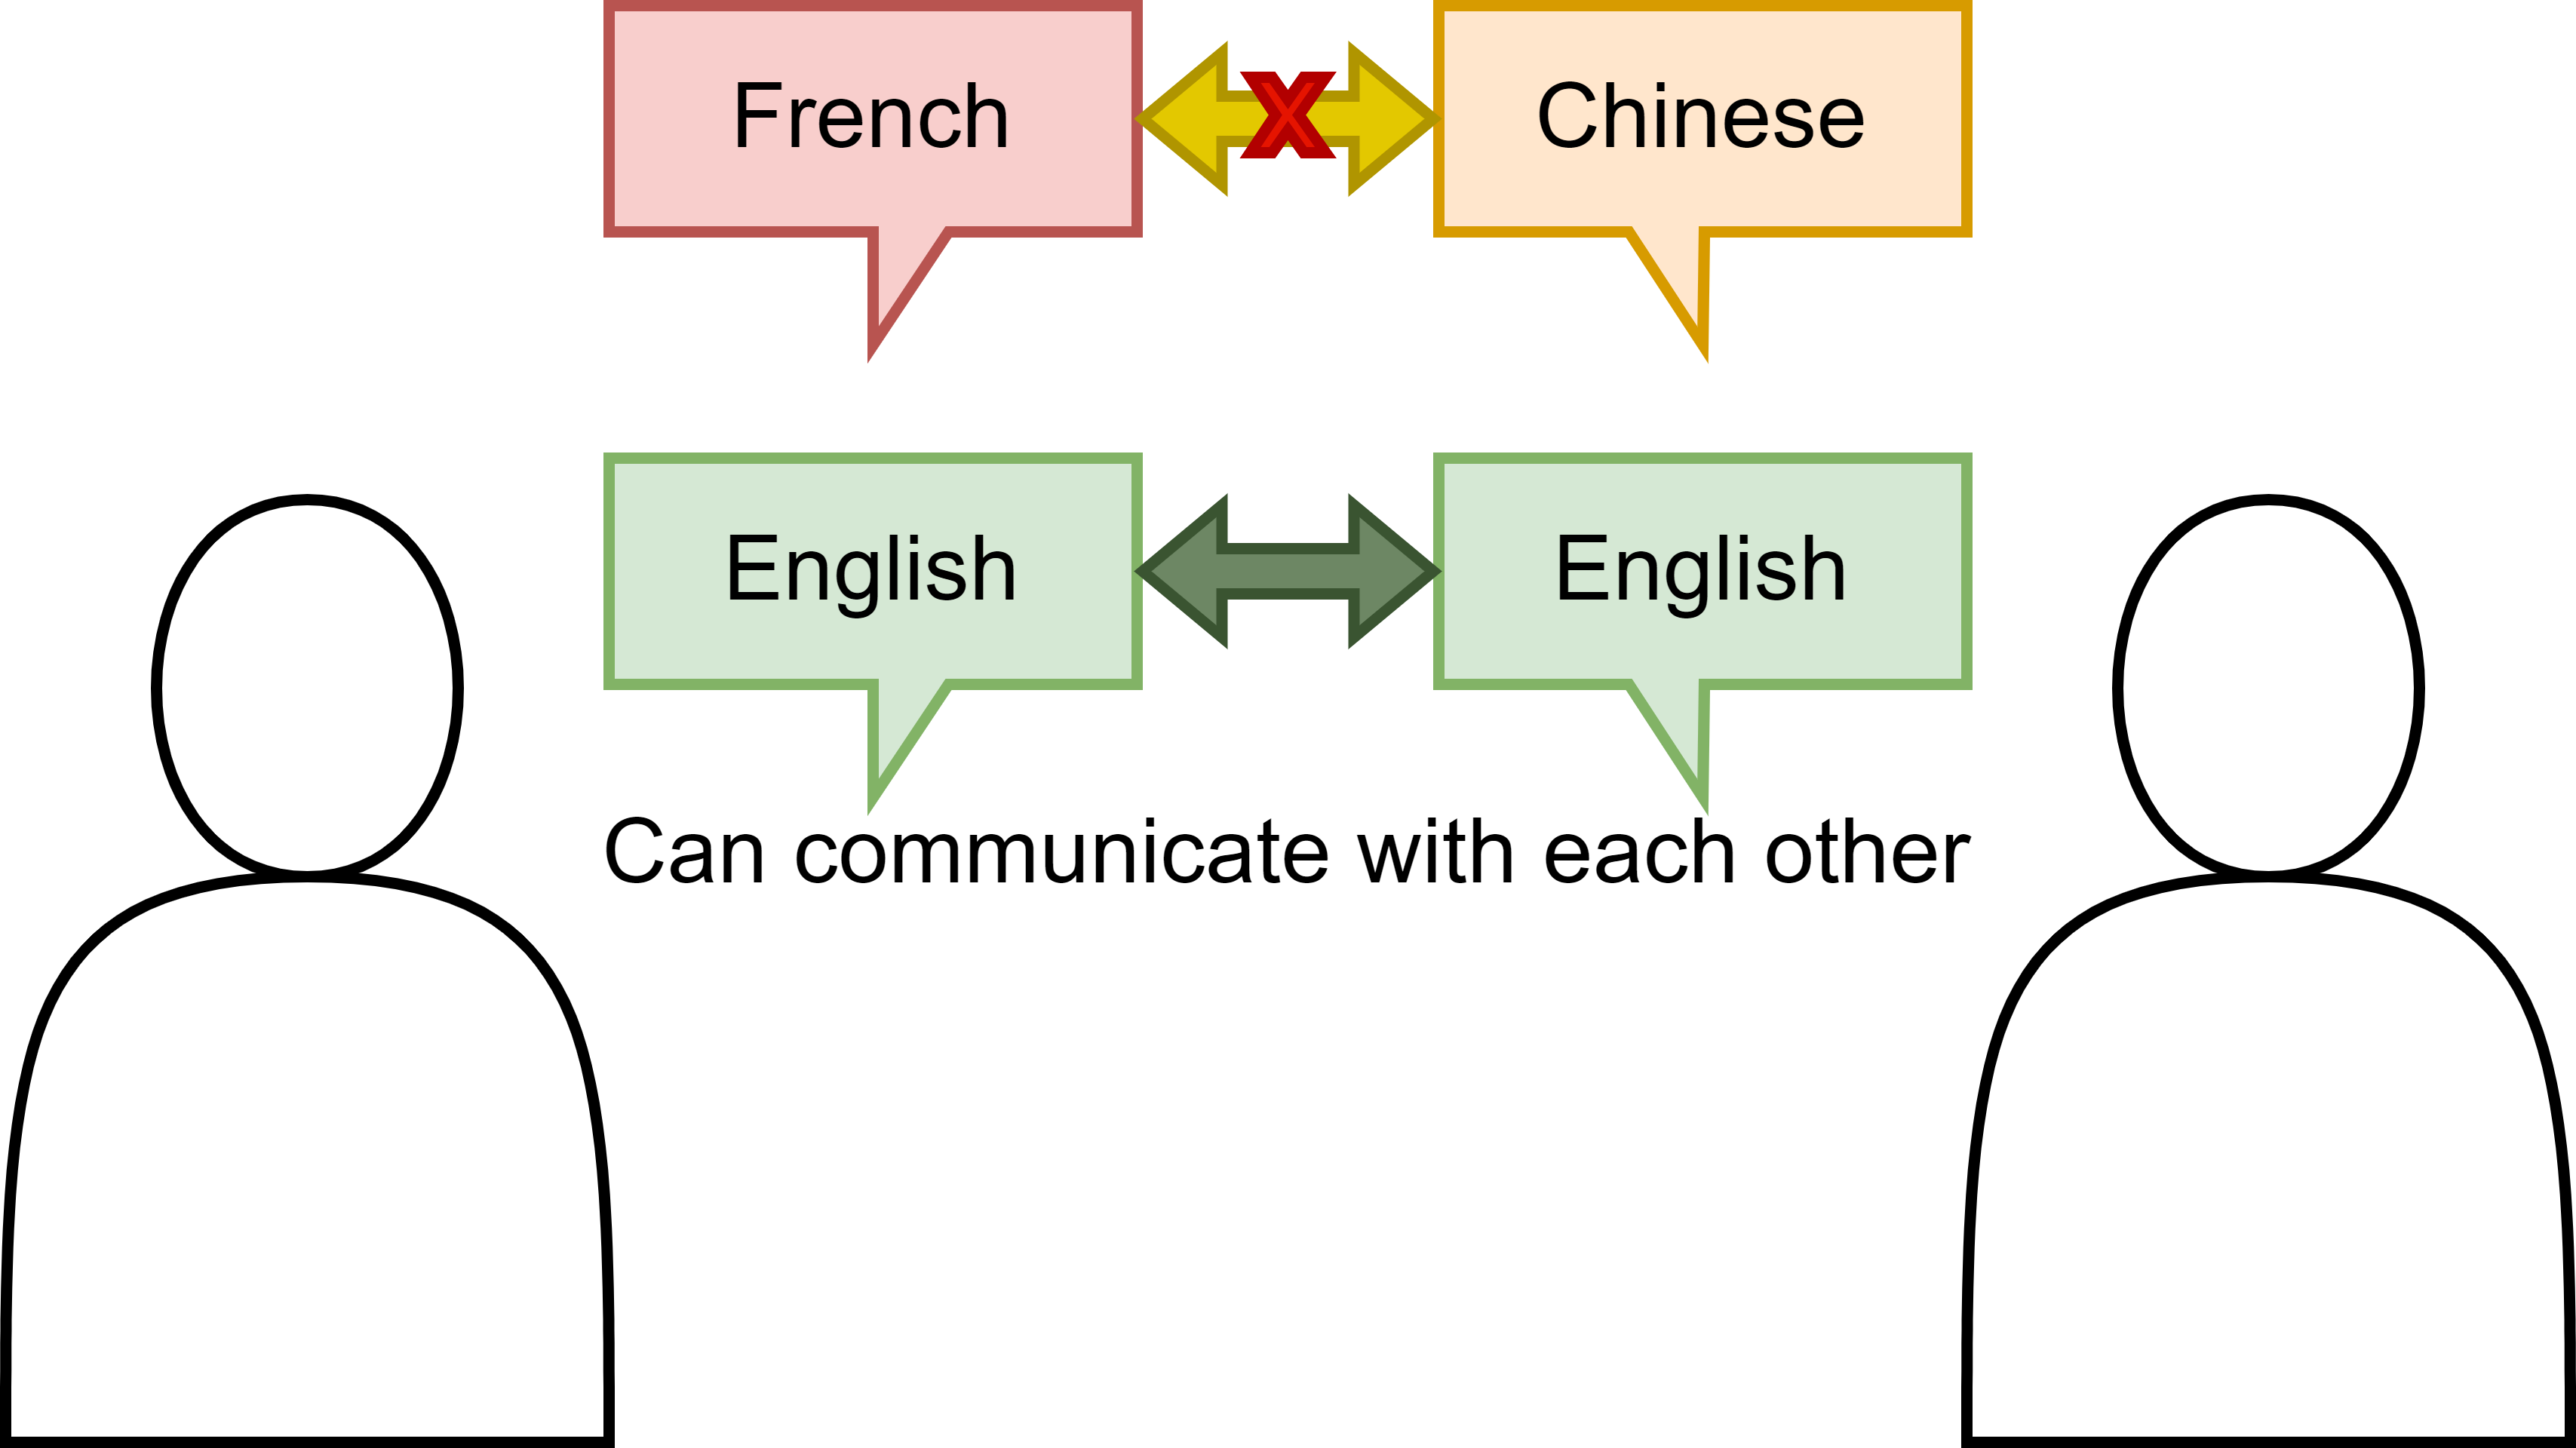
\includegraphics[width=0.56\textwidth]{images/CommunicationStandard.png}\\
	\caption[Compact Routing Example]%
          {Human communication with languages as a communication standard as an analogy for a communication standard for mobile robots}
	\label{fig:introduction__humanstandard}
\end{figure}

Different communication protocols and standards for industry 4.0 are under development \cite{sanneman_state_2020}. Information about the mobile robots such as manufacturer, model name, or actions can be exchanged with those protocols. To use a standard, the interfaces of the mobile robots need to be compliant with the interface the standard uses.  However, given no standard is yet dominant in the industry, most mobile robots are not compliant with a standard. To address the different external interfaces of the mobile robots a middleware is needed that enables communication through the different interfaces of the mobile robots and the interfaces of the application controlling the mobile robots.  Figure ~\ref{fig:introduction__humanstandardtranslator} on page ~\pageref{fig:introduction__humanstandardtranslator} shows the human analogy of such a middleware. A translator (blue rectangle) enables  communication between two people from different languages by translating the languages (one person symbolizes a mobile robot, and the other a controlling application). The translator is the analogy for the middleware to enable communication between a controlling application and a mobile robots with different interfaces. The languages can be translated directly by the translator, or it translates every language to an internal language before translating it further to another language (represented by the dotted rectangle). A middleware for mobile robots could use such an internal language module.

\begin{figure}[!ht]
	\centering
	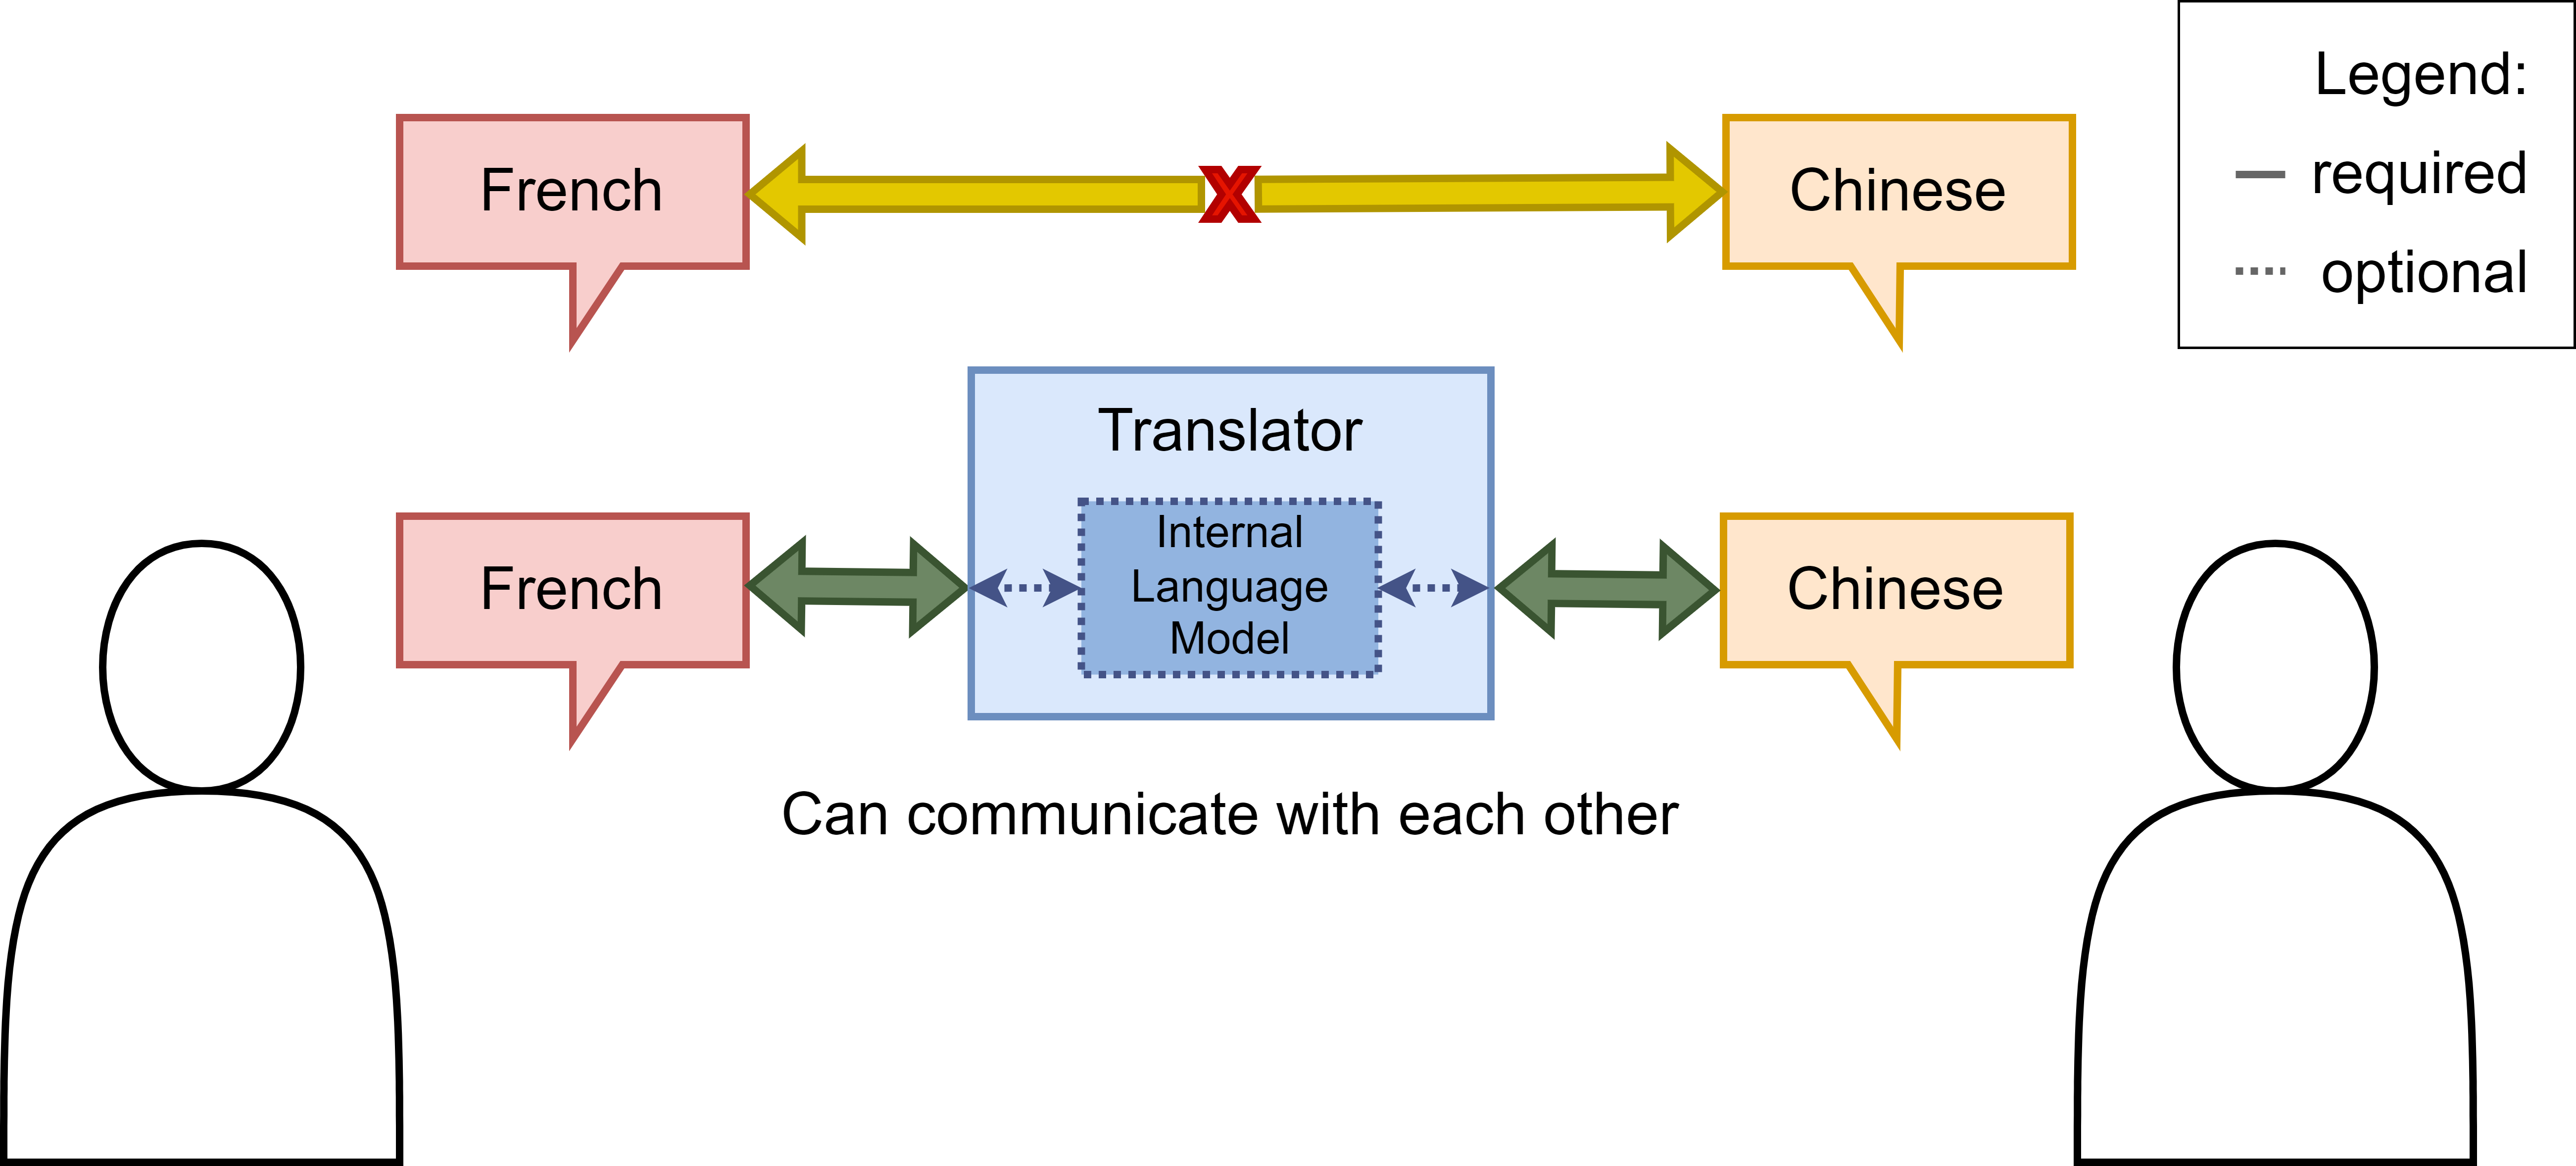
\includegraphics[width=0.86\textwidth]{images/CommunicationStandardTranslator.png}\\
	\caption[Compact Routing Example]%
          {Translator in human communication for translating languages as an analogy for an adapter for mobile robots' interfaces}
	\label{fig:introduction__humanstandardtranslator}
\end{figure}

\newpage

This thesis is written by Mai Khanh Isabelle Wilhelm at the SNET chair of the TU Berlin in cooperation with the BASF Group which is an industry leader in chemistry. The main goal of the thesis is to build a middleware that allows a superordinate application to control two mobile robots from different vendors. To control the mobile robots the Business Process Management (BPM) system PROCEED\footnote{Business Process Management system PROCEED \url{https://docs.proceed-labs.org/}} will be used. It has been developed at the SNET chair at TU Berlin. BPM systems aim to improve business processes by modeling, analyzing, optimizing, and automating the processes. 

Figure ~\ref{fig:introduction__middleware} on page ~\pageref{fig:introduction__middleware} shows a first, general concept for this thesis. The controlling application PROCEED (blue rectangle) will communicate with the mobile robots from different vendors through the middleware (red rectangle) and vice versa. The middleware has on one side an interface towards PROCEED following a communication standard (represented by the Standardized Interface) and has on the other side adapters for every mobile robot to address the different, proprietary interfaces (represented by the Vendor-dependent Interface) of two mobile robots: the MiR100\footnote{MiR100 \url{https://www.mobile-industrial-robots.com/solutions/robots/mir100/}} (yellow rectangle) and the RoboMaster S1\footnote{RoboMaster S1 \url{https://www.dji.com/de/robomaster-s1}} (green rectangle).  The middleware, therefore, acts as a translator for the interface of a controlling application (e.g. PROCEED) and the mobile robots from different vendors. 

\begin{figure}[!ht]
	\centering
	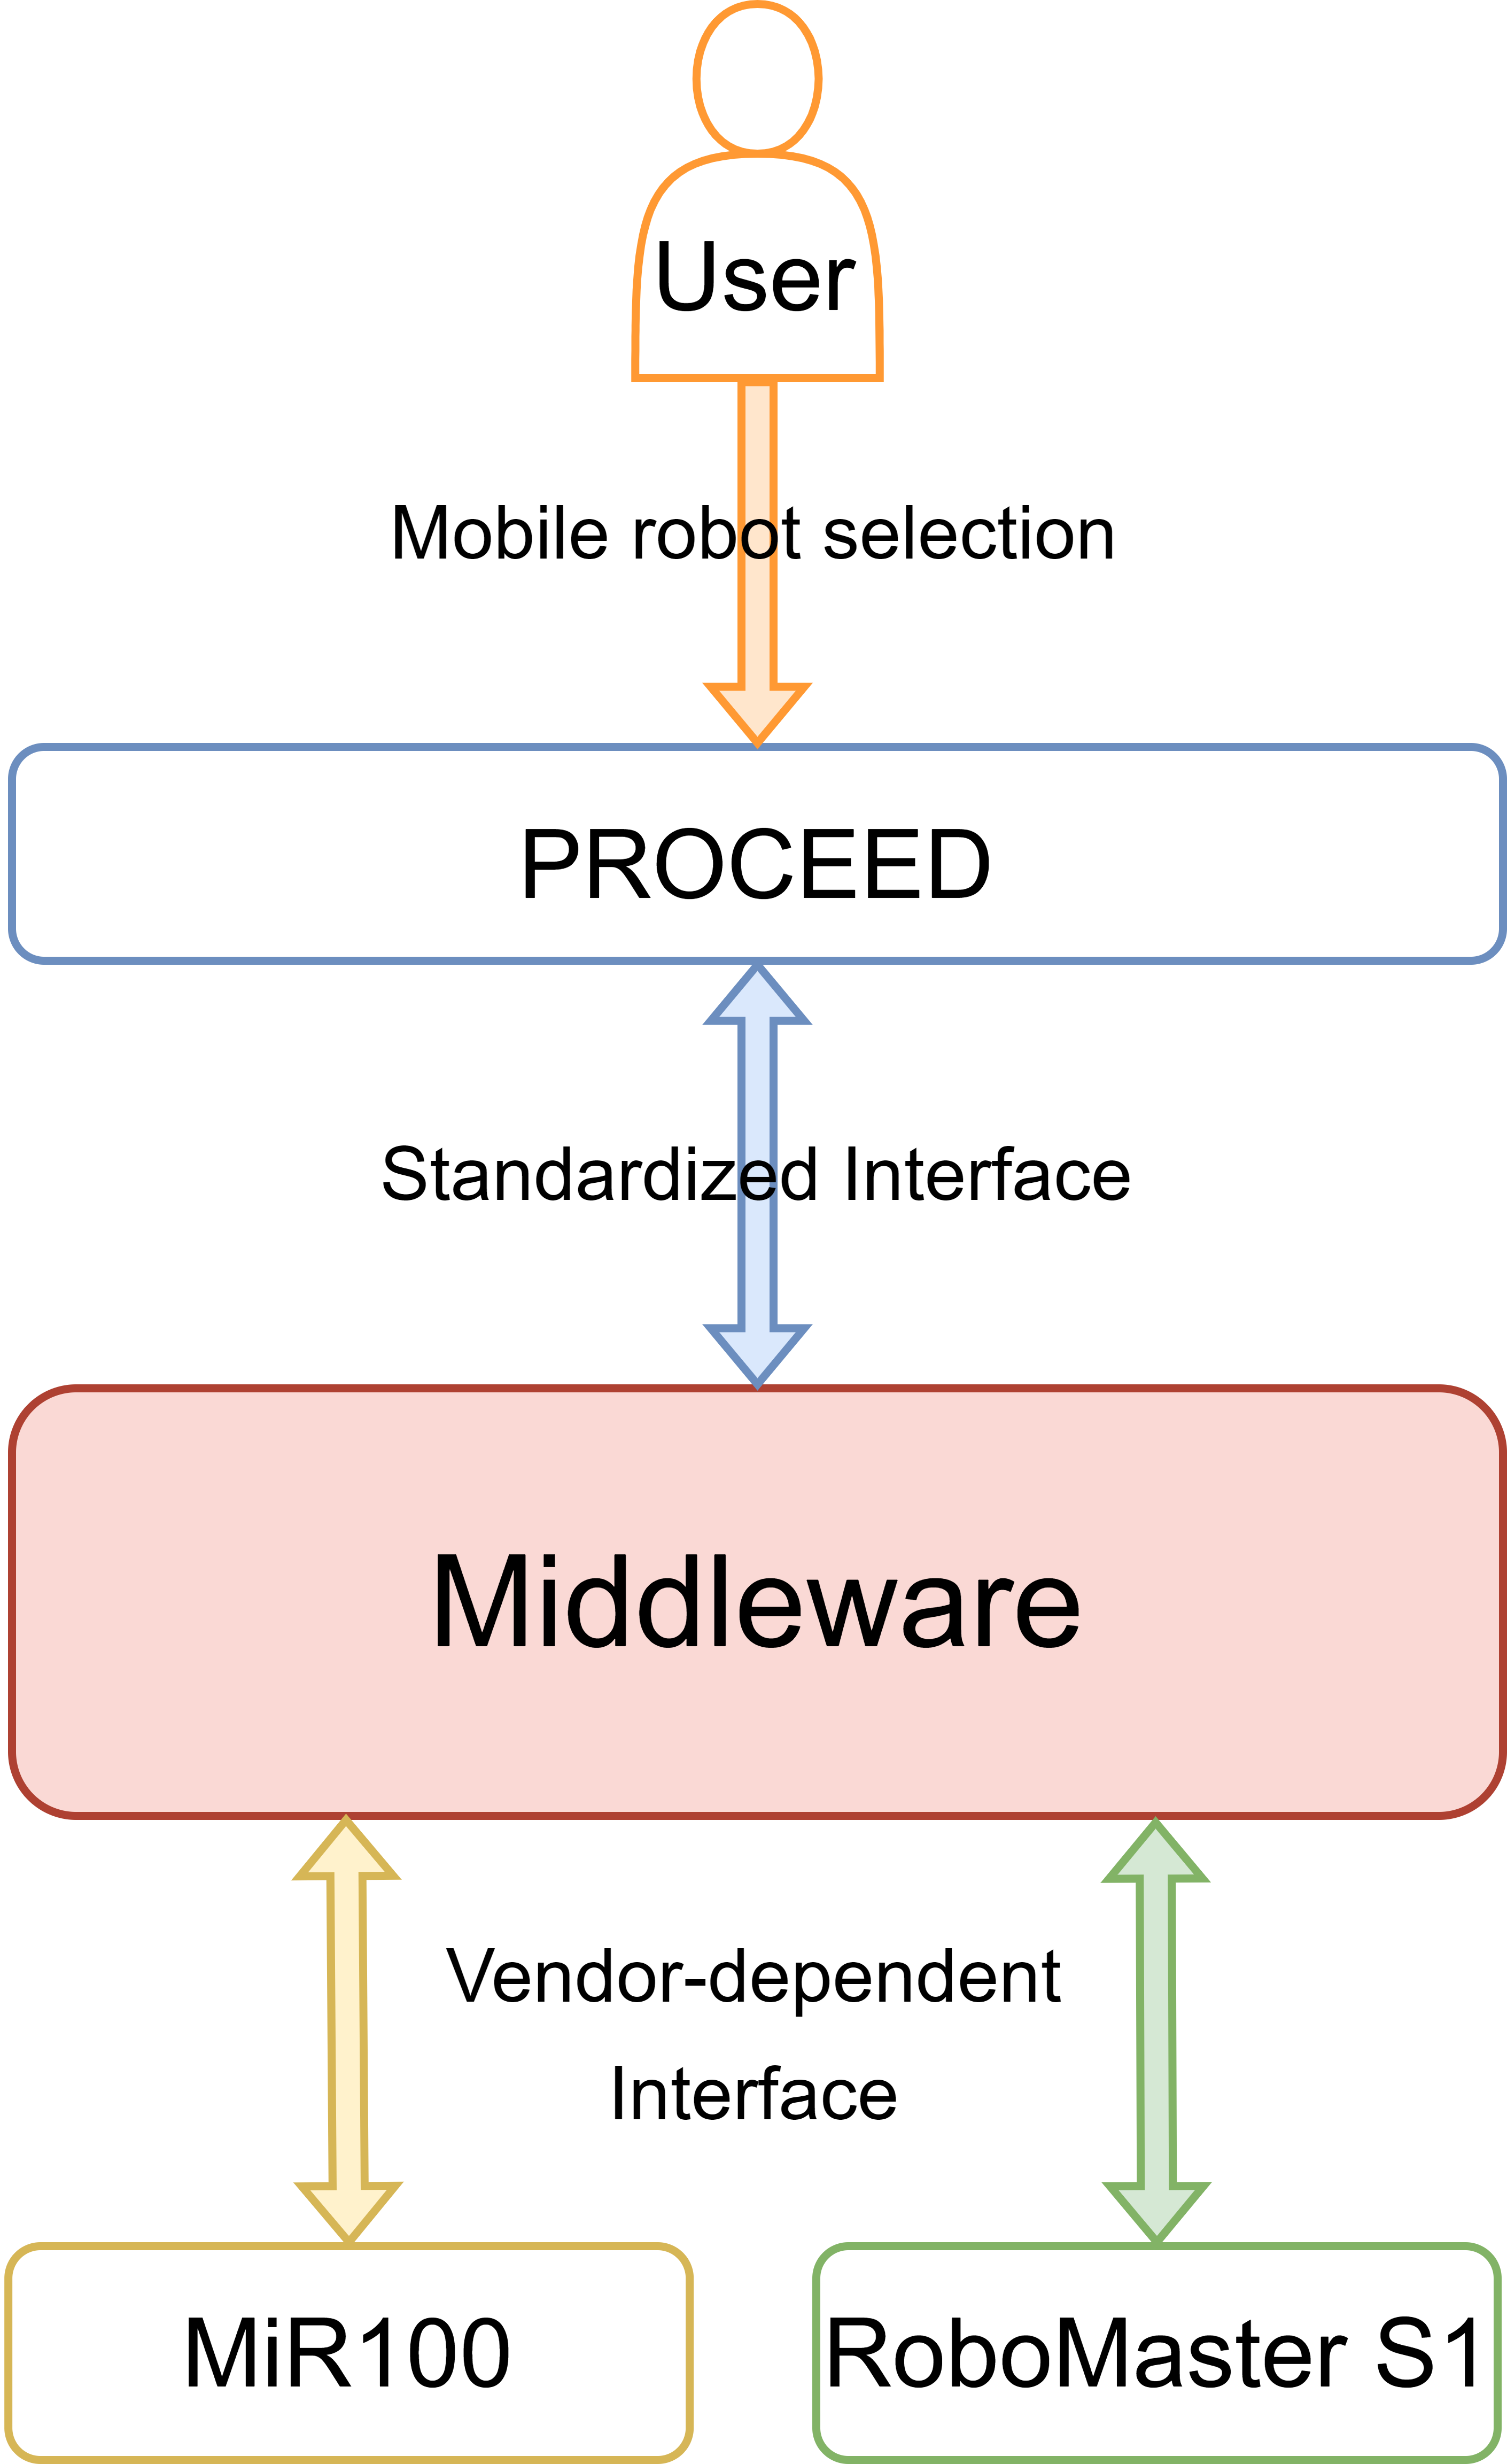
\includegraphics[width=0.4\textwidth]{images/Middleware.png}\\
	\caption[Compact Routing Example]%
    {General concept of a middleware to enable multi-vendor mobile robot communication}
	\label{fig:introduction__middleware}
\end{figure}

\newpage
Another aim of the thesis is to select suitable mobile robots for the process manually in PROCEED. This manual user interaction is represented with the orange user symbol in figure ~\ref{fig:introduction__middleware}. Several mobile robots may be suitable for a task, hence, it needs to be decided which mobile robot should execute the task. Selecting the most suitable robot for a task such as the mobile robot which is the closest, reduces the costs and time of the process. This thesis is working toward easily integrating multiple mobile robots from different vendors into an automated system without complex configurations (“plug and play”). To achieve that adapters for different mobile robot interfaces can be integrated into the middleware. Hence, mobile robots can be used more flexibly in production plants which will help the industries to stay competitive.

\section{Use Cases Description}
Through the middleware, PROCEED will communicate to the mobile robots to drive from point-to-point, as well as to pick up and drop a load. One use case must (required use case) and the second may (optional use case) be realized with the middleware.
 \begin{itemize}
   \item \textbf{ PROCEED must be able to select a suitable mobile robot from all available mobile robots from different vendors} \hfill \\
Thanks to standardized communication interfaces PROCEED can easily request information from the mobile robots to determine during runtime and during the configuration phase which mobile robots are suitable for the upcoming task. The user can then choose a mobile robot from the list of suitable mobile robots, or the most suitable mobile robot can be selected automatically.
   \item \textbf{ The middleware may allow a mobile robot to pick up a load from a mobile robot from a different vendor or drop it on that mobile robot} \hfill \\
In addition to picking up a load from a stationary target such as a shelf or dropping it on itself, the mobile robot may pick up a load from a second mobile robot or drop it on the second mobile robot. To guarantee a smooth interaction, the mobile robots need to communicate their status to each other. Possible solutions for this communication are manual user input or automatic feedback from the mobile robots. The BASF Group has been working since 2021 on such a use case. In their process, a manual input signalizes to the mobile robots when they can interact with each other. Using a middleware that bridges the communication gap between two different, proprietary interfaces would allow to fully automate such processes.
  \end{itemize}

\section{Research Questions}
From the first draft of a concept arise the following research questions:
\begin{itemize}
   \item \textbf{RQ1 - How to design a middleware to enable communication of mobile robots from different vendors and a controlling application such as PROCEED?} \hfill \\ 
The focus of this research question is to simplify the integration of multiple mobile robots from different vendors. This research question also covers the state-of-the-art for multi-vendor mobile robots approaches and it leads to the following research questions.
\begin{itemize}

     \item \textbf{RQ1}
     \item \textbf{RQ1}
     \item \textbf{RQ1}
     \item \textbf{RQ1}
     \item \textbf{RQ1}
     \item \textbf{RQ 2.4 - With which principle: push or pull should the middleware communicate with the mobile robots?} \hfill \\ 
The push principle in communication is that the mobile robots communicate status information such as their current position to PROCEED through the middleware without any request for information. This information can be sent cyclic, e.g. the mobile robot can update its information to the middleware every 10 seconds. The other principle is the pull principle. For this principle, messages are sent when they have been requested by the superordinate entity (PROCEED). It needs to be identified which principle will be used for the mobile robots and the middleware.
   \item \textbf{RQ1}
\end{itemize}
   \item \textbf{RQ2 - How can the middleware be integrated into the BPM system PROCEED to allow communication between this application and multi-vendor mobile robots} \hfill \\ 
The middleware should be able to run alone as well as be integrated into PROCEED. This research will answer further sub-questions:
   \begin{itemize}
     \item \textbf{RQ 2.1 - How can mobile robots be integrated into PROCEED?} \hfill \\ 
The mobile robots can be integrated into PROCEED, or into the middleware. It needs to be evaluated which approach is better suitable for this thesis. It is also of high interest whether the adapter for the mobile robots should be directly on the mobile robots themselves or whether they should be integrated into the middleware.
     \item \textbf{RQ 2.2 - Where can suitable robots manually be selected in PROCEED?} \hfill \\ 
PROCEED has two major software components. It needs to be evaluated which of the two options is better to select a suitable mobile robot for the process.
     \item \textbf{RQ 2.3 - When should the suitable mobile robot manually be selected in PROCEED?} \hfill \\ 
Whether a mobile robot can complete a task depends on its functionalities such as whether it can carry a load. This can be decided during the configuration phase. During run-time, the middleware can check whether mobile robots that have been selected during the configuration phase are online. Further, during run-time mobile robots can be selected depending on their battery level and their distance from the current location of the mobile robot to the start point of the task for the mobile robot. PROCEED models processes with the graphical language Business Process Model and Notation (BPMN). Figure ~\ref{fig:introduction__bpmn} on ~\pageref{fig:introduction__bpmn} represents an example of a BPMN diagram, modeling the process for a mobile robot to fetch a package. It needs to be identified at which point of the diagram the manual selection will take place. One possible option is that the manual selection takes place at the beginning of the task "Robot fetches package" when the task is in the state ready. Adding the task "Preparing for package pick-up" in which  the manual selection takes place is another option.
\begin{figure}[!ht]
	\centering
	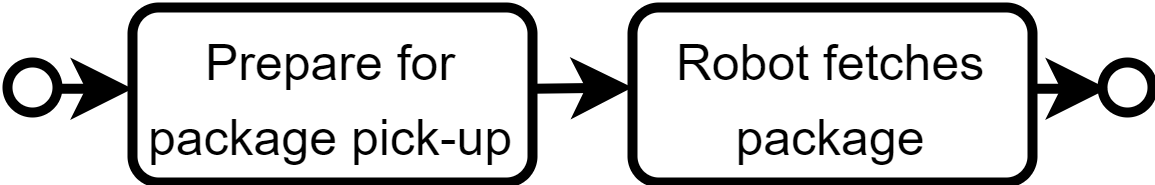
\includegraphics[width=0.5\textwidth]{images/BPMN.png}\\
	\caption[Compact Routing Example]%
          {Example of a BPMN diagram that models the process for a mobile robot to fetch a package}
	\label{fig:introduction__bpmn}
\end{figure}
     \item \textbf{RQ 2.4 - What are the benefits of a central and decentral approach?} \hfill \\ 
PROCEED has the option to run centrally, as well as decentrally. Centrally means that one system acts as a central coordinator for the entire process. Decentralized systems do not have such a central coordinator. In this case, mobile robots can communicate directly and therefore in a decentralized manner. This research will try to cover the advantages and challenges of direct and indirect communication between mobile robots from different vendors. It needs to be identified what the benefits of both approaches are and which approach will be used in this thesis.
   \end{itemize}
\end{itemize}

\section{Task Description}
The tasks of this thesis can be categorized into three groups: what must, what should, and what may be completed. In the following list, the tasks of the thesis are described where the numbering corresponds to a prioritization of the tasks.

What \underline{must} be done:
\begin{enumerate}
   \item \textbf{A superordinate entity must be able to control at least two mobile robots from different vendors through the middleware} \hfill \\
	The thesis aims to develop a middleware through which a controlling application such as PROCEED and mobile robots from different vendors can communicate with each other. To control the mobile robots, PROCEED must be able to tell the mobile robots which actions to perform and the mobile robots must be able to communicate to PROCEED their status. Therefore, the middleware must enable bidirectional communication to two mobile robots from different vendors, adapted to their external interfaces. This task consists of multiple subtasks:
   \begin{enumerate}
     \item\textbf{At least two specific mobile robots must be registered}
To be able to control specific mobile robots, they must be registered on either PROCEED or the middleware.
     \item\textbf{PROCEED must be able to trigger the action to drive from point-to-point to the mobile robots} \hfill \\
Mobile robots can execute different actions. One of those actions is the ability to drive. It must be possible to communicate through the middleware to the mobile robots to execute a drive action.
     \item\textbf{The mobile robots must be able to communicate to PROCEED their status information} \hfill \\
To control the mobile robots, PROCEED requires status information of the mobile robots. This status information needs to be communicated through the middleware. It can be sent periodically from the mobile robots, or it can be sent after PROCEED requests it.
     \item\textbf{PROCEED must be able to request the proprieties of the mobile robots} \hfill \\
PROCEED requires information about the proprieties of the mobile robots such as dimensions, maximum speed, and payload to assign suitable tasks to the mobile robots.
   \end{enumerate}
     \item\textbf{Suitable robots must be selected via user input in PROCEED} \hfill \\
Selecting which mobile robot to use must be selected according to the mobile robot’s functionalities e.g. whether it can pick up a load, and what its dimensions are. Other criteria for choosing a suitable mobile robot can be the distance to the task or the battery level. This selection option must be displayed in PROCEED and be manually chosen by the user. For that, it needs to be decided where the user input in PROCEED will take place.
   \item \textbf{The middleware must communicate to PROCEED using existing communication protocols and standards} \hfill \\ 
	The middleware has two interfaces: one interface towards the controlling application PROCEED, and adapters towards the mobile robots. The interface towards PROCEED must follow an existing communication protocol or standard. This enables the potential of the middleware by making it easier to add further controlling applications to the middleware. If no suitable standard exists, the minimum requirements for such a standard must be identified.
   \item \textbf{The middleware must be scalable for further mobile robots} \hfill \\ 
	The middleware must be able to easily extend further mobile robots from different vendors with different interfaces. Each different, proprietary interface can be addressed through an adapter. The middleware must have the option to easily embed more adapters into it.
\end{enumerate}

What \underline{should} be done:
\begin{enumerate}
   \item \textbf{PROCEED should handle exceptional cases when no suitable mobile robots are available} \hfill \\ 
	If no mobile robot which meets the functional and technical requirements exists, an error message should be sent out. Examples of no suitable mobile robot being available could be both mobile robots being out of battery or both mobile robots not having the function the task requires them to have e.g. picking up a too heavy load.
   \item \textbf{PROCEED should be able to communicate to the mobile robot further actions} \hfill \\ 
	After having added the possibility that the mobile robots perform a drive action, further actions that are defined in the chose communication standard such as charge, pick up and drop should be added to PROCEED and the middleware. It is desired that further actions can be added, when the standard is developped further.
\end{enumerate}

What \underline{may} be done:
\begin{enumerate}  
   \item \textbf{PROCEED may be able to select a suitable robot depending on its functional requirements or data automatically} \hfill \\ 
	A suitable robot may be selected automatically depending on the functionalities needed to complete the task. If several robots are suitable an algorithm that selects one needs to be implemented. That algorithm may include the robot which is the closest or which has the highest battery level. Further, a random selection may also be suggested.
   \item \textbf{The middleware may be able to integrate other applications besides PROCEED} \hfill \\ 
	The middleware may be able to easily extended with further applications that control the mobile robots. Applications that are addressable of the same interface and protocol as PROCEED are desired to be integrated into the middleware. Those applications allow testing whether the mobile robots can be controlled with any application that uses the chosen standard.
   \item \textbf{PROCEED may be able to communicate to one mobile robot to fetch a load from a second mobile robot or to drop the load on it} \hfill \\ 
	In an industrial process, it is desired that mobile robots can directly interact with each other by one picking up a load from another mobile robot or by dropping the load on top of the other mobile robot. The mobile robot may be able to communicate through the middleware to the other mobile robot when they are ready to interact with another mobile robot and when they have completed the interaction.
\end{enumerate}



\chapter{Related Work}
\label{cha:relatedwork}

!!!Eine Einleitung hier ... therefore a lot of research ... a special focus is !!!

SECTION STANDARD
corba
vda 5050

\section{Middleware}
To bridge mobile-robot specific hardware and software, the paper \cite{utz_miro_2002} suggests the middleware Miro which is based on the CORBA standard. It consist of three architectural layers.
\chapter{Concept and Design}
\label{cha:conceptanddesign}

Describe the concept and the design of your work here
\chapter{Implementation}
\label{cha:implementation}

Describe the details of the actual implementation here...
\chapter{Evaluation}
\label{cha:evaluation}

The evaluation of the thesis should be described in this chapter
\chapter{Conclusion}
\label{cha:conclusion}

Describe what you did here

%--------------------------------------------------------------
% TABLES, FIGURES, BIBLOGRAPHY AND APPENDICES
%--------------------------------------------------------------
\backmatter

% Lists of tables and figures
\listoftables
\listoffigures

% Bibliography
\setwidesite{}						% Set page to be wider for bibliography
\markboth{Bibliography}{bibliography}
\label{cha:bibliography}
\bibliographystyle{IEEEtran}
\bibliography{bibliography.bib}

% Use following to separate online (websites) and offline (books, papers) sources
%\printbibliography[heading=offline,filter=offline]
%\printbibliography[heading=online,filter=online]

\begin{appendices}
	\chapter{Appendix 1}
\label{appendix:listing1}

\lstset{language=PHP}
\begin{lstlisting}
for($i=1; $i<123; $i++)
{
    echo "work harder! ;)";
}
\end{lstlisting}
	% \input{content/99_appendices/a02_listings}
	% \input{content/99_appendices/a03_listings}
\end{appendices}

\end{document}
